\section{Attention Mechanism}
\label{sec:nlp_attention}
The attention mechanism mimics the retrieval of a value $v_i$ for a query $q$ based on a key $k_i$ in database.
$$attn(q, k, v) = \sum_i sim(q,k_i)\times v_i$$
\begin{figure}[h]
	\centering
	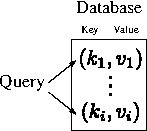
\includegraphics[scale=2.0]{./images/transformer/attention_database.pdf}
	\caption{The most similar key will be selected by measuring a similarity between a query and a key.}
\end{figure}

\begin{figure}[h]
	\centering
	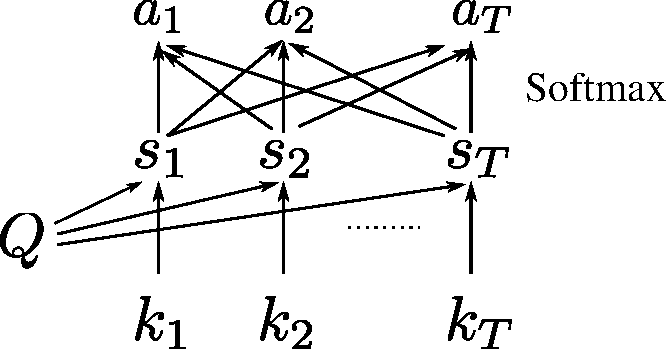
\includegraphics[scale=0.8]{./images/transformer/attention.pdf}
	\caption{The similarity $s_t$ is computed by a query and keys}
\end{figure}
There are several choices for a similarity function.
\begin{itemize}
	\item $q^Tk_i$: dot product.
	\item $\frac{q^Tk_i}{\sqrt{d}}$: scaled dot product $\to$ reduce the variance of the final attention weights. 
	\item $q^TWk_i$: general dot product.
	\item $w_q^Tq+ w_k^Tk_i$: additive similarity.
\end{itemize}
Finally, the attention score can be computed by using a softmax:
$$a_i = \frac{\exp(s_i)}{\sum_j \exp(s_j)}$$

\section{Transformer}
\label{sec:nlp_transformer}

Self-attention:
$$attn(Q,K,V) = softmax(\frac{Q^TK}{\sqrt{d_k}})V$$
Masked attention (cross-attention. Self-attention in decoder):
$$\textrm{MA}(Q,K,V) = softmax\bigg(\frac{Q^TK+M}{\sqrt{d_k}}\bigg)V,$$
where $M$ is a matrix of 0 and $-\infty$. Note that $-\infty$ will make $exp$ term to be zero.


\begin{figure}[h]
	\centering
	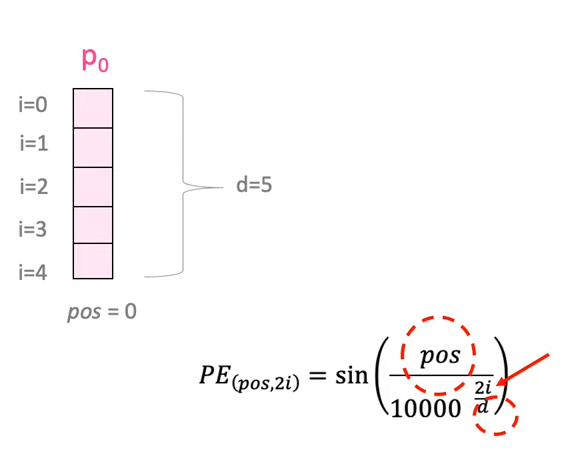
\includegraphics[scale=0.6]{./images/transformer/positional_1.png}
	\caption{Positional embedding.}
\end{figure}
